\section{Problem}
 \begin{wrapfigure}{r}{0.18\columnwidth}
\vspace{-2.5em}
		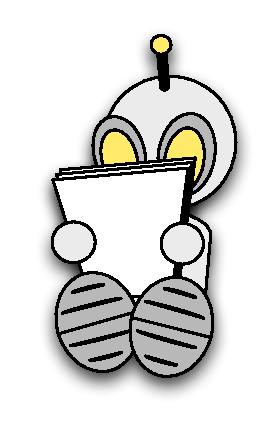
\includegraphics[width=0.18\columnwidth]{diagrams/robot_reading.pdf}
\vspace{-2em}
 \end{wrapfigure}
Single agent pathfinding is one of the classical problems of Computer Science.
The aim is to find the shortest possible path between a pair of locations 
on a known map. 
It has many real-world applications in areas as diverse as logistics, 
robotics and most recently video games.
\newline \newline
In the context of single-agent pathfinding the seminal A* algorithm 
\cite{hart68} is regarded as the gold standard. 
Though many attempts have been made to improve on its performance success always 
comes at a price: for example, by trading solution
optimality for speed~\cite{botea04} or otherwise using significantly more memory than A*~\cite{sturtevant09}.
In this work we develop a new technique for speeding up A* which is fast,
optimal and requires no significant extra memory compared to standard
A*.
Our method is based on the observation that for any given pair of locations on a
grid map there are usually many symmetric paths of optimal length. 
We attempt to identify and eliminate such symmetries and in the process create
a smaller map which is faster to search.
Our approach is specific to solving pathfinding problems in 4-connected grid
maps -- a common encoding which appears often in the academic literature and in
the pathfinding systems of many modern video games.

\subsection{Grid Maps}
A grid map is a simple 2-dimensional representation of terrain in which every
tile is either marked as traversable or not traversable.
Agents then move from one traversable tile to the next according to a series of 
simple transition rules.
In the case of 4-connected grids we are restricted to moving in the 4 cardinal
directions (i.e. no diagonal moves are allowed).

\begin{figure}[h]
\vspace{1em}
	\centering
	\subfigure[Robotic navigation] {
	\label{fig:maze}
		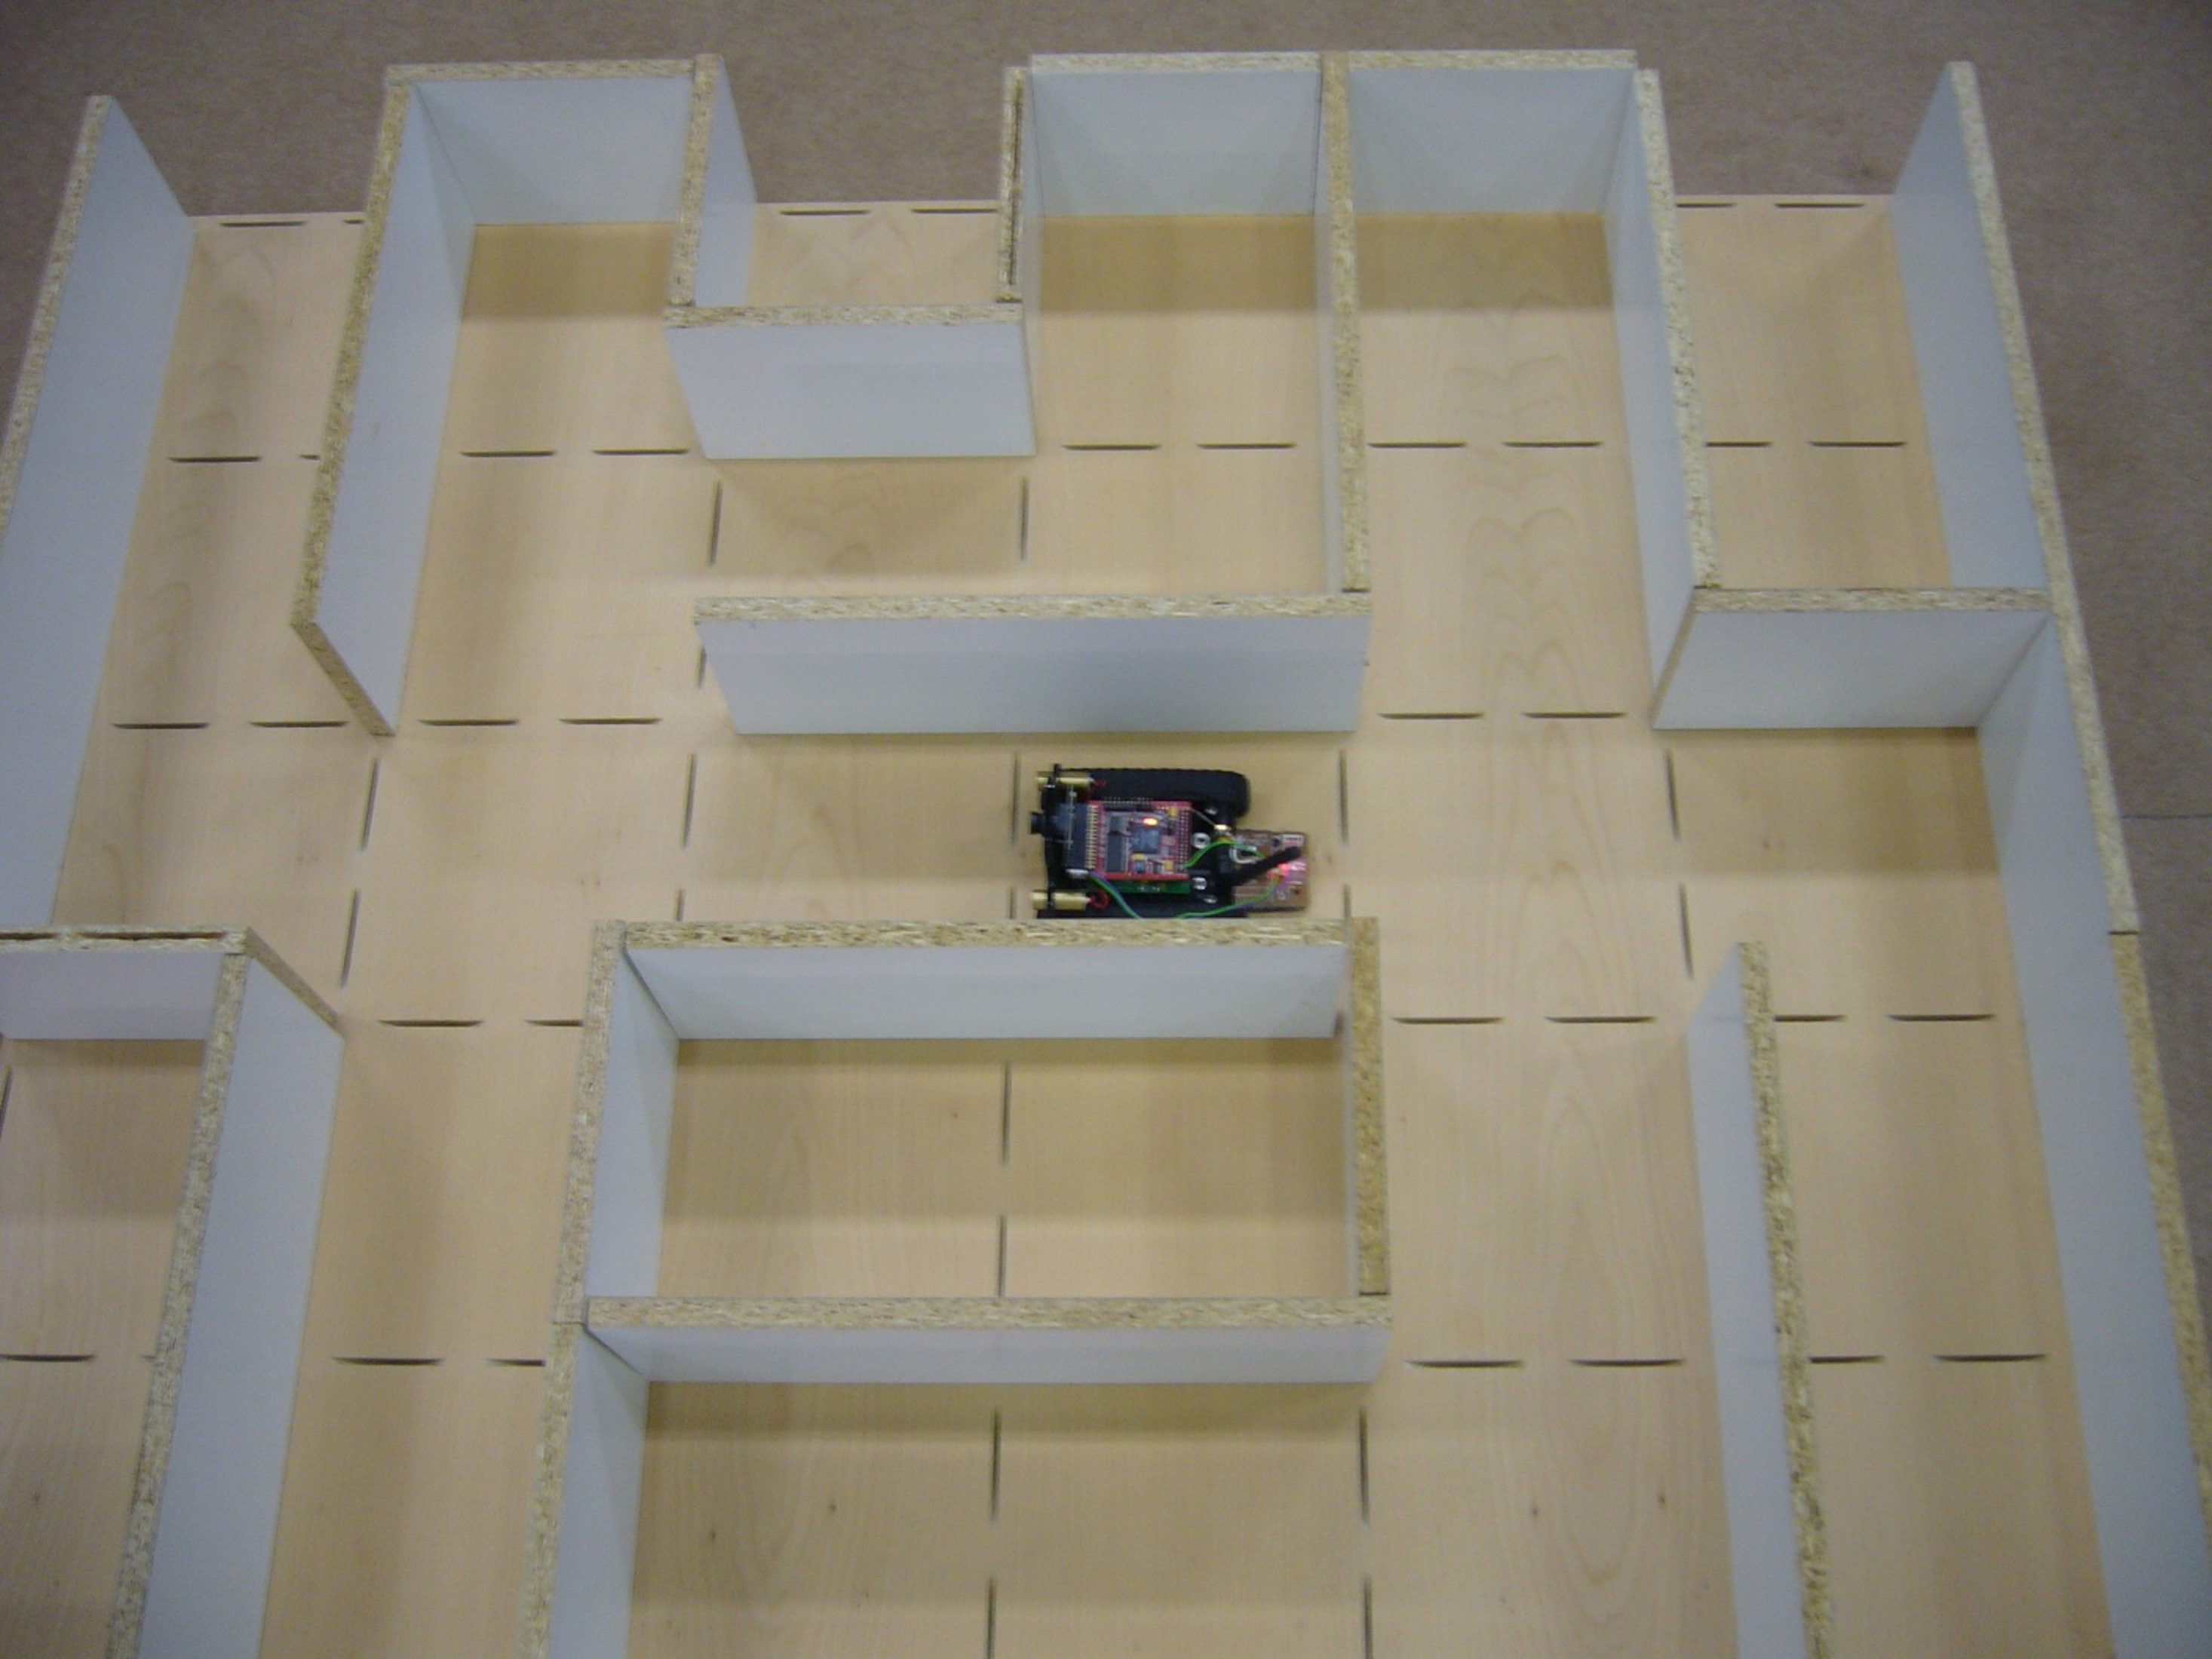
\includegraphics[width=0.47\columnwidth]{diagrams/maze.pdf}
	}
	\subfigure[Video games (shown: Icewind Dale 2)] {
	\label{fig:iw2}
		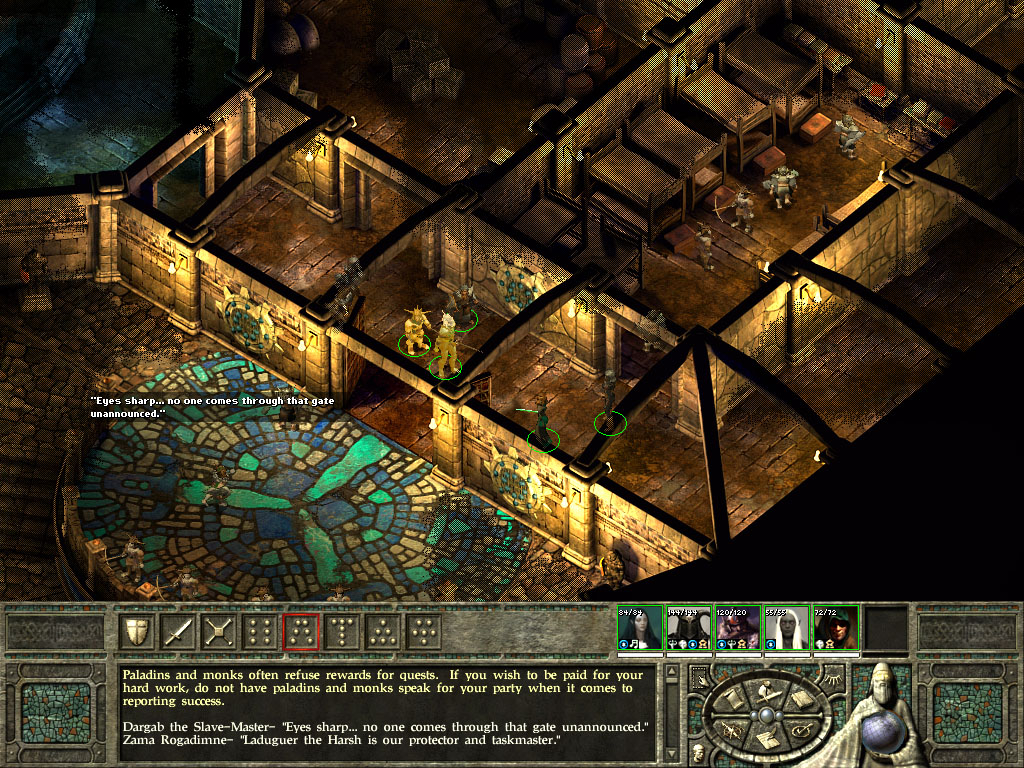
\includegraphics[width=0.47\columnwidth]{diagrams/iwdale.jpg}
	}
\vspace{-0.5em}
{
\small \caption{Applications areas where grid maps are commonly used.}
}
\vspace{1em}
 \end{figure}

Though less popular than the 8-connected variant (in which diagonal moves are
allowed) 4-connected grids appear regularly in the literature \cite{yap02} and in the pathfinding
systems of many modern video games. 
Some recent examples include Square Enix's \emph{Heroes of Mana} (released for the Nintendo DS),
Astraware's \emph{My Little Tank} (iPhone) and Atari's \emph{Dragon Ball Z: Legacy of Goku} 
(Gameboy Advance). 
